% !Mode:: "TeX:UTF-8" 



\BiSection{2.2}{Figures}

解:

(1)对于NFET:

$g_m=\sqrt{2\mu_nC_{ox}\frac{W}{L}I_D}=3.66\frac{mA}{V}$

\color{blue}{
	\{
	$C_{ox},\mu_n\text{见习题2.1中,单位换算}\frac{A \cdot s}{V}=F$
	
		\begin{figure}[H] %H为当前位置,!htb为忽略美学标准,htbp为浮动图形
		\begin{minipage}{\linewidth}
			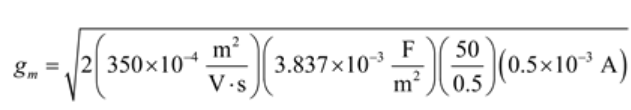
\includegraphics{2.2-1}
		\end{minipage}
	\end{figure}
	
	\begin{figure}[H] %H为当前位置,!htb为忽略美学标准,htbp为浮动图形
		\begin{minipage}{\linewidth}
			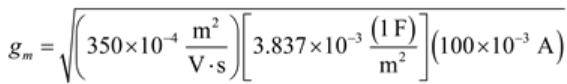
\includegraphics{2.2-2}
		\end{minipage}
	\end{figure}
			\begin{figure}[H] %H为当前位置,!htb为忽略美学标准,htbp为浮动图形
		\begin{minipage}{\linewidth}
			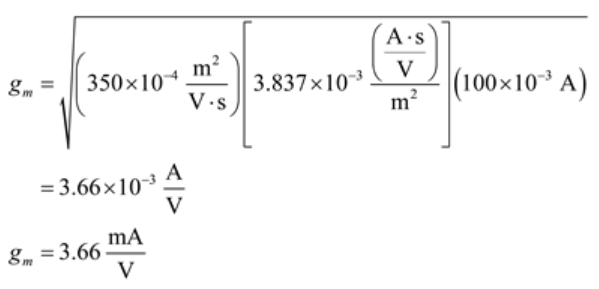
\includegraphics{2.2-3}
		\end{minipage}
	\end{figure}
	\}
	
	
}

\color{black}{
$r_o=\frac{1}{\lambda_n I_D}=20k\Omega$

}


\color{blue}{
	\{
	$\lambda_n \text{见表2.1中,单位换算}\frac{V}{A}=\Omega$
	
	\begin{figure}[H] %H为当前位置,!htb为忽略美学标准,htbp为浮动图形
		\begin{minipage}{\linewidth}
			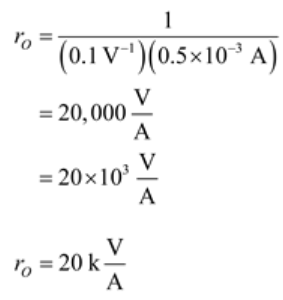
\includegraphics{2.2-4}
		\end{minipage}
	\end{figure}
	
	\}
	
	
}

\color{black}{
	本征增益$g_mr_o=73.2\frac{V}{V}$
	
	
	
	(2)对于PFET:
	
	$g_m=\sqrt{2\mu_pC_{ox}\frac{W}{L}I_D}=1.96\frac{mA}{V}$
	
	$r_o=\frac{1}{\lambda_p I_D}=10k\Omega$
	
	本征增益$g_mr_o=19.6\frac{V}{V}$
	
}